\documentclass{standalone}
\usepackage{tikz}
\usepackage{pgfplots}
\usepackage{xcolor}

\pgfplotsset{
    compat=1.18,
    grid style={gray!30},
    legend style={
        at={(0.98,0.98)},
        anchor=north east,
        fill=white,
        draw=black,
        font=\small
    }
}

\begin{document}
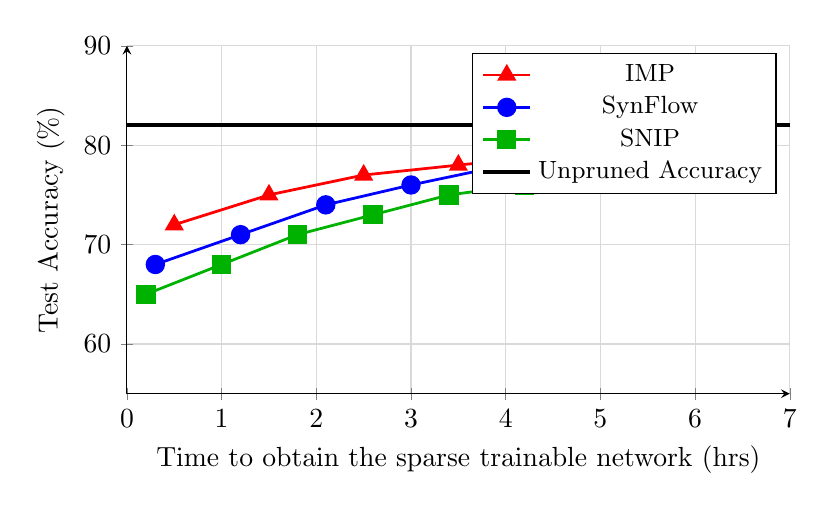
\begin{tikzpicture}
\begin{axis}[
    width=10cm,
    height=6cm,
    xlabel={Time to obtain the sparse trainable network (hrs)},
    ylabel={Test Accuracy (\%)},
    xmin=0, xmax=7,
    ymin=55, ymax=90,
    grid=both,
    grid style={gray!30},
    legend style={
        at={(0.98,0.98)},
        anchor=north east,
        fill=white,
        draw=black,
        font=\small
    },
    tick align=outside,
    axis lines=left
]

% IMP data (red triangles)
\addplot[red, mark=triangle*, mark size=3pt, line width=1pt] 
coordinates {
    (0.5,72) (1.5,75) (2.5,77) (3.5,78) (4.5,79) (5.5,80) (6.5,81)
};
\addlegendentry{IMP}

% SynFlow data (blue circles)
\addplot[blue, mark=*, mark size=3pt, line width=1pt] 
coordinates {
    (0.3,68) (1.2,71) (2.1,74) (3.0,76) (4.0,78) (5.0,79) (6.0,80)
};
\addlegendentry{SynFlow}

% SNIP data (green squares)
\addplot[green!70!black, mark=square*, mark size=3pt, line width=1pt] 
coordinates {
    (0.2,65) (1.0,68) (1.8,71) (2.6,73) (3.4,75) (4.2,76) (5.0,77)
};
\addlegendentry{SNIP}

% Unpruned Accuracy (black horizontal line)
\addplot[black, line width=1.5pt, no marks] 
coordinates {
    (0,82) (7,82)
};
\addlegendentry{Unpruned Accuracy}

\end{axis}
\end{tikzpicture}
\end{document}